%%%%%%%%%%%%%%%%%%%%%%%%%%%%%%%%%%%%%%%%%%%%%%%%%%%%%%%%%%%%%%%%%%%%%%
% How to use writeLaTeX: 
%
% You edit the source code here on the left, and the preview on the
% right shows you the result within a few seconds.
%
% Bookmark this page and share the URL with your co-authors. They can
% edit at the same time!
%
% You can upload figures, bibliographies, custom classes and
% styles using the files menu.
%
% Texto de até 4 páginas (utilizando o template da SBC) descrevendo:
% A escolha do(s) algoritmo(s) e sua adequação ao problema proposto.
% Os hiperparâmetros definidos e justificativa para os valores escolhidos.
% Discussão dos resultados obtidos e possíveis melhorias.
% Texto explicativo e documentação (30%)
% O texto explica com clareza a escolha do modelo e os resultados obtidos.
% O código-fonte é bem documentado e organizado no repositório.
%
%%%%%%%%%%%%%%%%%%%%%%%%%%%%%%%%%%%%%%%%%%%%%%%%%%%%%%%%%%%%%%%%%%%%%%

\documentclass[12pt]{article}
\usepackage{sbc-template}
\usepackage{graphicx,url}

\graphicspath{{./fig/}}

\usepackage[brazil]{babel}   
\usepackage[utf8]{inputenc}  
     
\sloppy

\title{Busca de partículas exóticas com árvores}

\author{Guilherme Akira Demenech Mori\inst{1}, Bruno Bogaz Zarpelão\inst{1}, Sylvio Barbon Junior\inst{2}}

\address{Departamento de Computação -- Universidade Estadual de Londrina
  (UEL)\\
  Rodovia Celso Garcia Cid, PR 445 Km 380 -- 86.055-900 -- Londrina -- PR -- Brazil
  \nextinstitute
  Department of Engineering and Architecture -- University of Trieste (UNITS)\\
  Via Alfonso Valerio 6/1, 34127 -- Trieste -- Italy
  \email{\{akira.demenech,brunozarpelao\}@uel.br, sylvio.barbonjunior@units.it}
}

\begin{document} 
\maketitle

\begin{abstract}
	The pursuit of discovery and the challenge of identifying exotic particles in high-energy particle colliders drive the use of machine learning techniques.
	Boosted decision trees and shallow neural networks are commonly employed, which require artificial variables to model nonlinear behaviors that are difficult to learn.
	This study aims to provide a user-friendly interface for exploring and comparing various decision tree classification models and for examining the significance of artificial variables built by researchers for the development of these models.
\end{abstract}
     
\begin{resumo} 
	O interesse na descoberta e a dificuldade de identificação de partículas exóticas em colisores motivam a utilização de técnicas de aprendizado de máquina.
	É comum a utilização de árvores de decisão e redes neurais rasas, que necessitam de variáveis artificiais modelando comportamentos não-lineares de difícil aprendizado.  
	Este trabalho tem como objetivo fornecer uma interface amigável para se explorar e comparar diferentes modelos de classificação por árvores de decisão e se observar a significância das variáveis artificiais desenvolvidas pelos pesquisadores para o aprendizado desses modelos.
\end{resumo}


\section{O problema e os algoritmos}
% A escolha do(s) algoritmo(s) e sua adequação ao problema proposto.
% O texto explica com clareza a escolha do modelo e os resultados obtidos.


Identificar processos sobre um grande fundo ruidoso é o desafio dos \textit{datasets} HIGGS \cite{higgs_280} e SUSY \cite{susy_279}.    
Desenvolvidos para testar a utilização de aprendizado profundo, eles incluem variáveis artificiais inseridas para auxiliar as técnicas de aprendizado menos poderosas que eram utilizadas até então \cite{Baldi_2014}.   
 
As principais abordagens, segundos os autores, eram redes neurais \textit{feed-forward} com uma única camada oculta e árvores de decisão com \textit{boost}. 
O trabalho original também menciona uma certa relutância por parte dos físicos em aceitar as limitações das redes neurais rasas e que eles tentam ajudar seus modelos combinando as variáveis detectadas não-linearmente com inspiração em modelos físicos.
A proposta testada e apresentada pelos autores é de que técnicas de aprendizado profundo podem descobrir os comportamentos complexos sem o auxílio dessas variáveis artificiais manualmente criadas e os resultados demonstraram melhoria na classificação.  

Árvores de decisão, bem como seus \textit{ensembles} com e sem \textit{boost} (modelos mencionados pelo trabalho dentre as técnicas utilizadas tradicionalmente na identificação dos sinais), permitem a verificação da importância de cada variável no processo de classificação.
Essa importância permite aos usuários entender quais funções não-lineares complexas construídas por pesquisadores são mais impactantes ou mais auxiliam a diferenciação de processos de fundo do sinal de interesse.  

Assim, tendo em vista essa transparência, neste trabalho escolhemos as árvores de decisão, o \textit{ensemble} \textit{random forest}, \textit{AdaBoost} e \textit{XGBoost}.
Foram selecionados os hiperparâmetros utilizados para poda das árvores (profundidade máxima e amostragem mínima para divisão e folha) e, nos modelos com \textit{boost}, aceleração de aprendizado (a taxa de aprendizado).
Os \textit{ensembles} também têm o hiperparâmetro adicional da quantidade de árvores da floresta.
Estão disponíveis, para comparação, os critérios de divisão e os divisores fornecidos pela biblioteca \textit{scikit-learn}.

Para explorar as diferenças entre os modelos (e os impactos da configuração dos hiperparâmetros neles) de aprendizado com árvores, bem como visualizar a utilização das variáveis observadas e das artificialmente derivadas das primeiras por esses modelos, o presente trabalho busca fornecer uma interface de fácil acesso, incluindo métricas e comparações úteis.

%\cite{higgs_280}
%\cite{susy_279}
%\cite{hepmass_347}

\section{Funcionamento e uso}

As responsabilidades foram organizadas em duas partes: aprendizado e interação.
No aprendizado estão as informações sobre os \textit{datasets} e a leitura deles, junto com os dados dos modelos e hiperparâmetros.
A interação é realizada pelo navegador \textit{web} com botões, seletores e campos de entrada, retornando os dados e gráficos de comparação.

Os componentes estão dispostos da seguinte maneira:

\begin{enumerate}
	\item O \textit{script} \texttt{back.py} importa os modelos e tem toda a organização para serem utilizados.
	Estão estruturados quais são os hiperparâmetros de cada um e quais são seus tipos e valores padrão.
	Os \textit{datasets} estão estruturados e descritos nele também.
	
	\item \texttt{front.py} tem as funções de interfaceamento entre \textit{Streamlit} e os modelos dispostos em \texttt{back.py} e é responsável pela criação dos gráficos com \texttt{matplotlib}.
	Ele tem a função \texttt{principal}, que chama todas as funções da interface de acordo com a sequência de interações com o usuário.
	
	\item \texttt{main.py} invoca a função \texttt{principal} de \texttt{front.py}.
\end{enumerate} 

Como as opções da interface estão estruturadas de maneira genérica, novos modelos ou \textit{datasets} podem ser adicionados inserindo suas informações em \texttt{back.py}. 
Sendo definidos a classe e os hiperparâmetros, os seletores e campos de entrada gerados por \texttt{front.py} os incluirão também.

A utilização segue uma sequência de formulário: 
pede-se as opções e dados e, a partir da submissão do usuário, é treinado e testado um modelo.

A apresentação dos resultados do teste é feita com alguns dados numéricos e gráficos comparando aos outros testes.
É possível visualizar as métricas de \textit{accuracy}, \textit{precision}, \textit{recall} e \textit{F1 score} para cada hiperparâmetro.
Os resultados dos testes realizados com um mesmo valor do hiperparâmetro visualizado serão apresentados como uma média no gráfico.

\section{Resultados}
% Os hiperparâmetros definidos e justificativa para os valores escolhidos.

Treinando os modelos com os dados de supersimetria (SUSY), é possível observar as importâncias das variáveis de entrada.
A Figura~\ref{impSUSY} mostra, para os modelos sem limitação de profundidade, que as variáveis observadas 6 e 0 e a variável artificial 9 tiveram maior relevância para as classificações de todos eles.
As variáveis artificiais 10, 11, 14, 16 e 17 tiveram flutuações na importância de um modelo para outro. 


% Discussão dos resultados obtidos e possíveis melhorias.

\begin{figure}[htb]
\centering
%\includegraphics[width=.49\textwidth]{Importância SUSY DT prof 5}
\includegraphics[width=.3\textwidth]{Importância SUSY DT prof None}
%\includegraphics[width=.49\textwidth]{Importância SUSY RF prof 5}
\includegraphics[width=.3\textwidth]{Importância SUSY RF prof None}
%\includegraphics[width=.49\textwidth]{Importância SUSY XG prof 5}
\includegraphics[width=.3\textwidth]{Importância SUSY XG prof None}
%\\ \hfill
\includegraphics[width=.3\textwidth]{Importância SUSY Ada prof None}
\caption{Gráficos de importância geradas para árvores de decisão, \textit{random forest}, \textit{XGBoost} e \textit{AdaBoost} com profundidades ilimitada com o \textit{dataset} SUSY}
\label{impSUSY}
\end{figure}



A Figura~\ref{SUSY} mostra as métricas de desempenho para os modelos com diferentes limitações de profundidade.
As métricas não mostraram diferenças significativas entre os melhores resultados de cada um, com cerca de 0.82 de precisão e 0.70 de \textit{recall} no máximo.
Essa observação de equivalência vai de encontro com o comentário dos autores, que mencionam uma espécie de estagnação nos avanços pelas técnicas até então adotadas terem mais ou menos o mesmo desempenho \cite{Baldi_2014}.

\begin{figure}[htb]
	\centering
	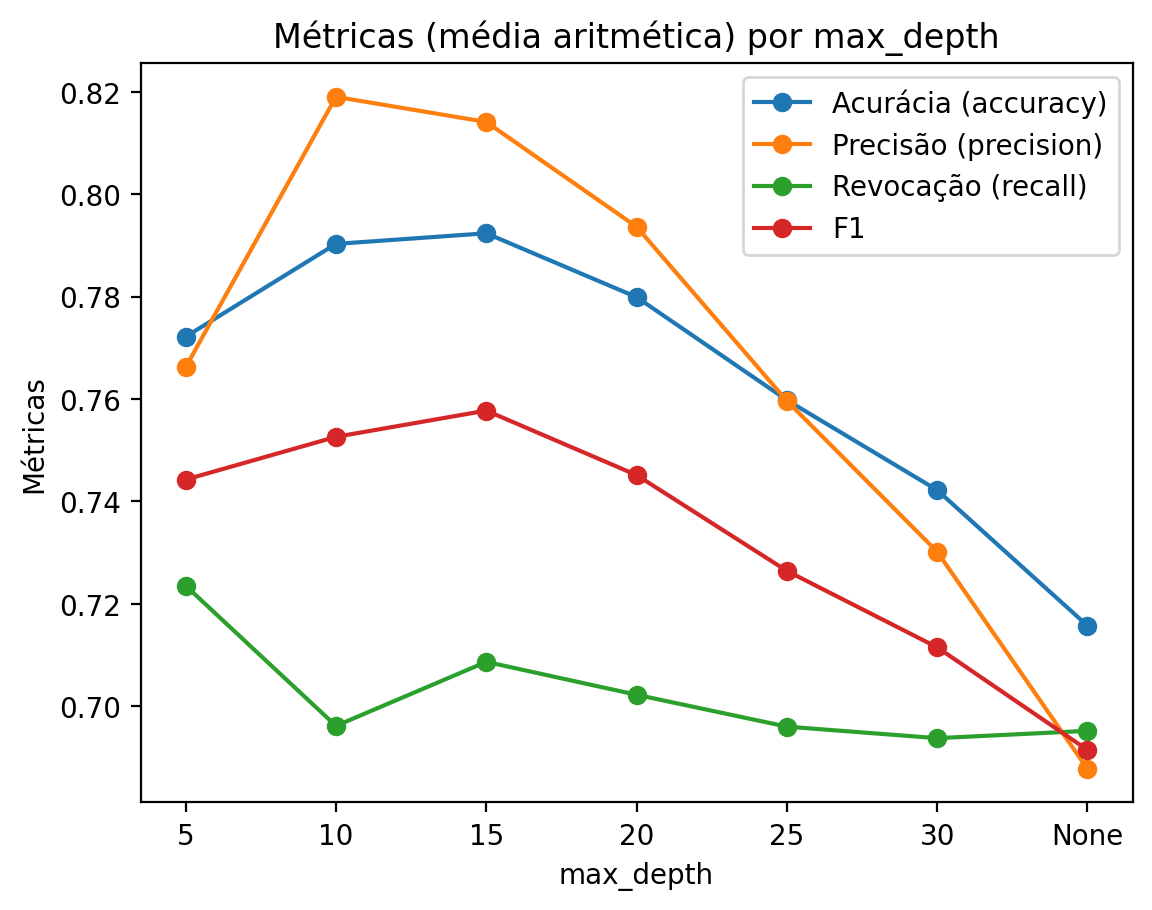
\includegraphics[width=.49\textwidth]{SUSY DT prof 5 10 15 20 25 30 None}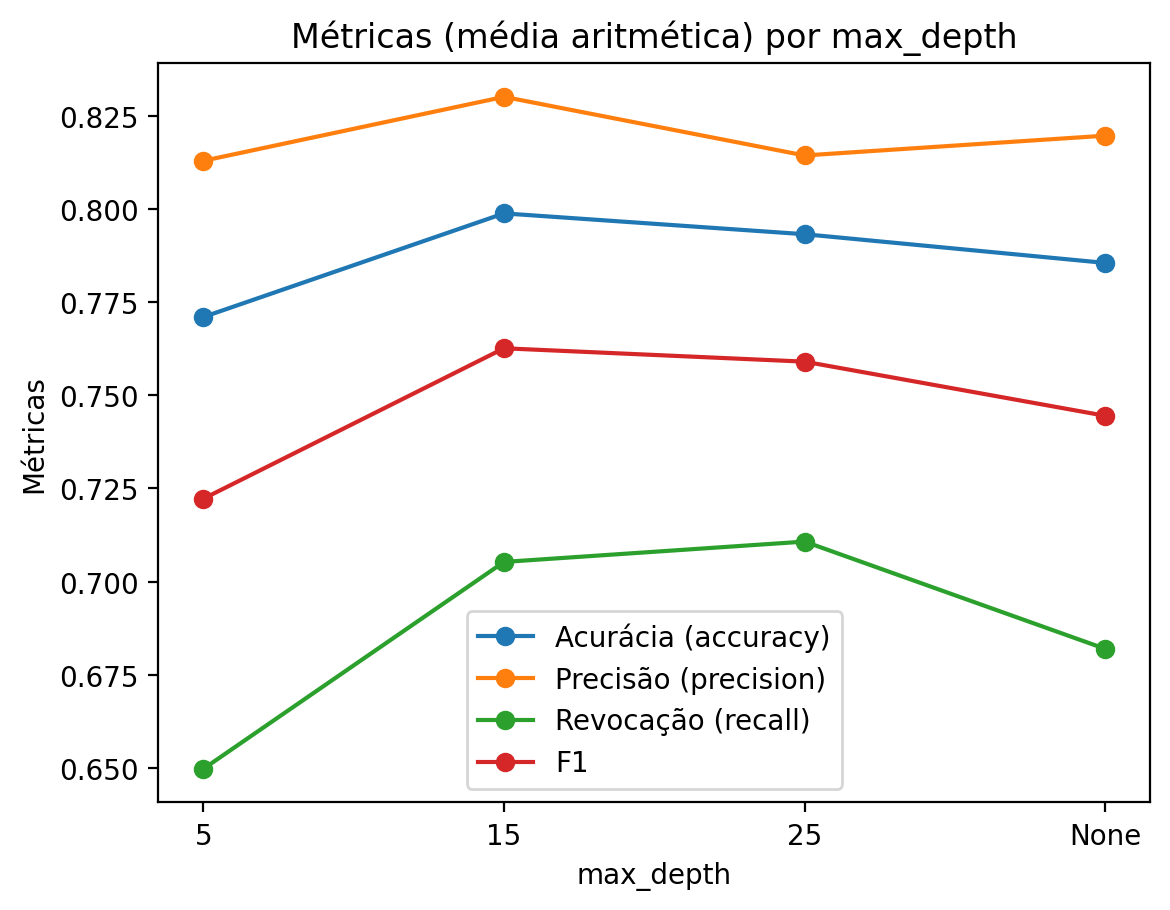
\includegraphics[width=.49\textwidth]{SUSY RF prof 5 15 25 None}
	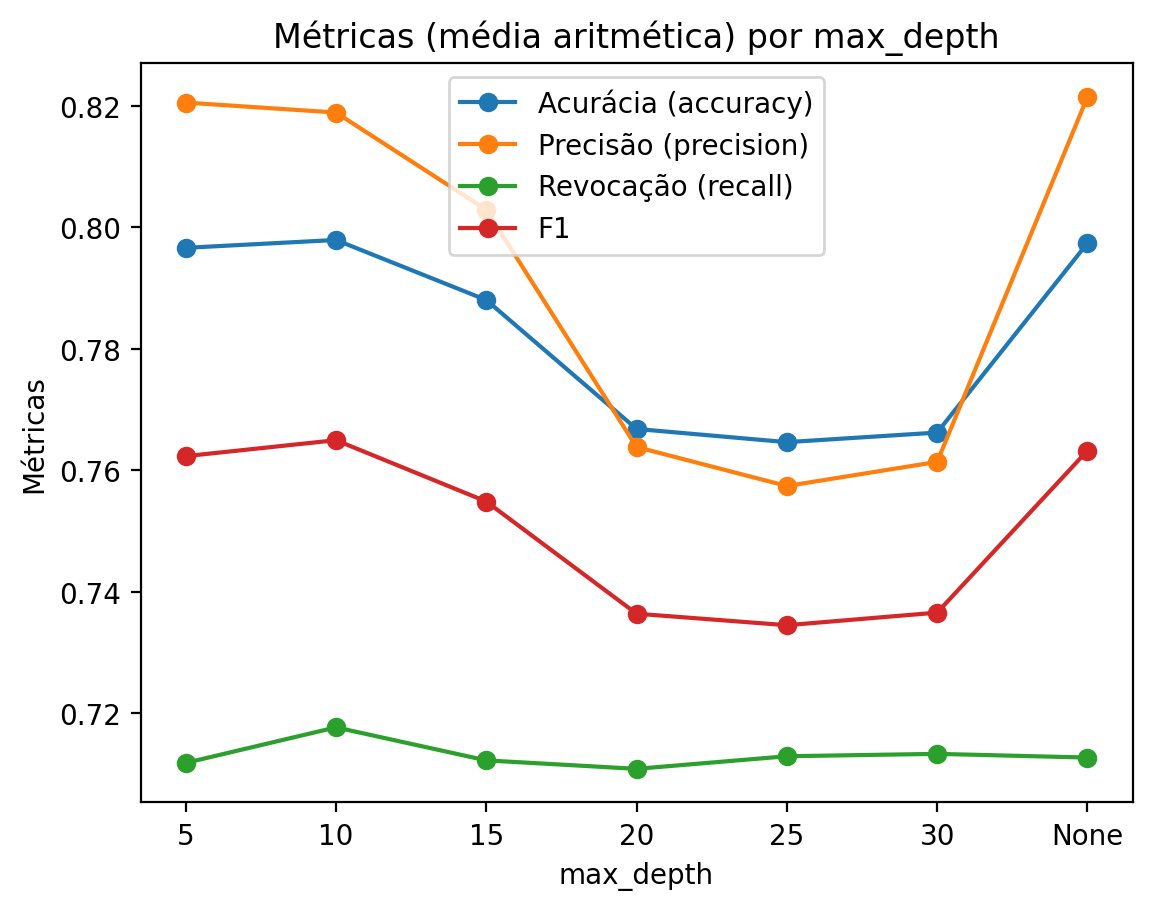
\includegraphics[width=.49\textwidth]{SUSY XG prof 5 10 15 20 25 30 None}
	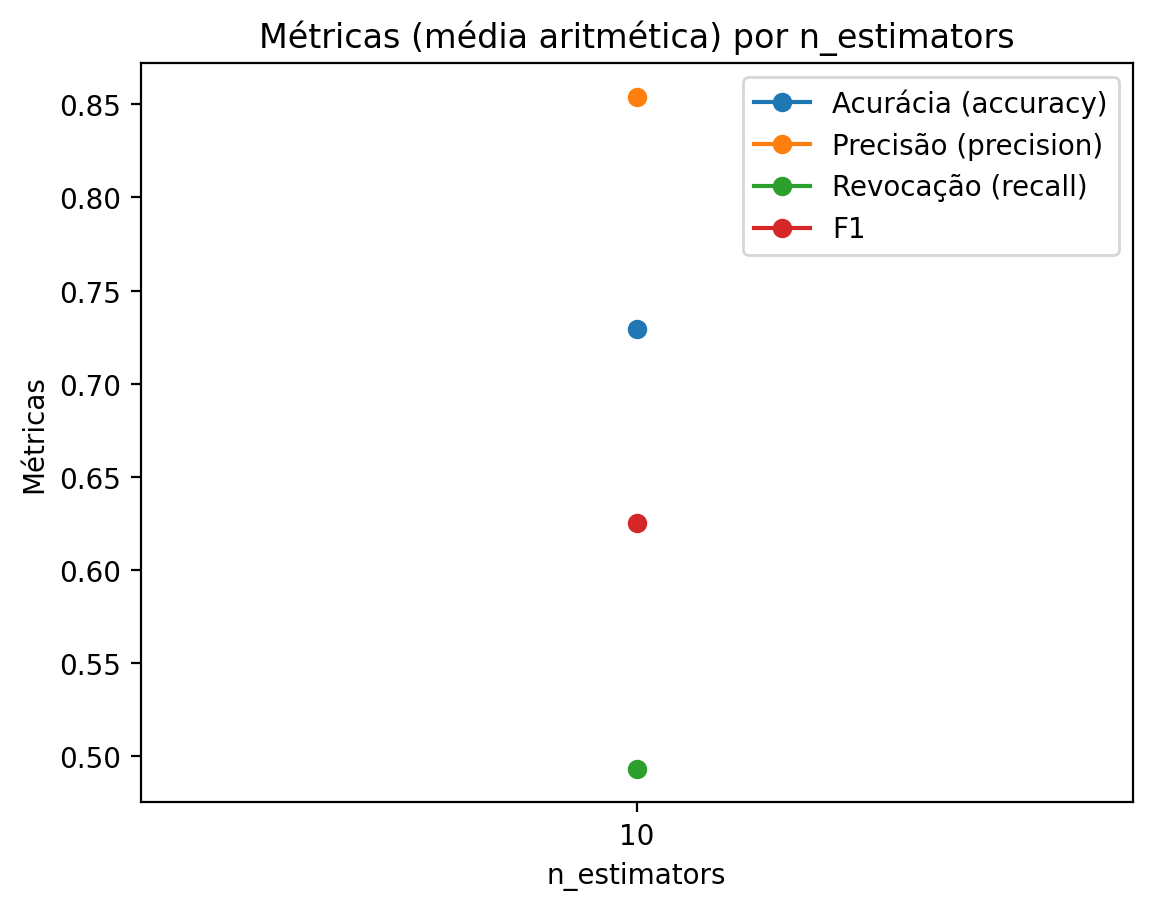
\includegraphics[width=.49\textwidth]{SUSY Ada n 10}
	\caption{Métricas das árvores de decisão, \textit{random forest}, \textit{XG Boost} e \textit{AdaBost} para diferentes valores de profundidade máxima}
	\label{SUSY}
\end{figure}




\section{Considerações finais}

Para usuários comuns, a limitação de processamento e memória de dispositivos pessoais dificulta a utilização. 
Computadores com até 8 GB de memória RAM não foram capazes de treinar modelos com os \textit{datasets} completos e mesmo computadores com mais memória e processadores modernos demoraram vários minutos para cada treinamento.
A execução na nuvem é um recurso necessário, especialmente se forem adicionados modelos de treinamento computacionalmente mais intenso, como as técnicas de \textit{deep learning} utilizadas no artigo original.

A inclusão do \textit{dataset} HEPMASS \cite{hepmass_347} também seria interessante. 
Para isso seria preciso generalizar mais a organização dos dados dos \textit{datasets} para permitir arquivos com cabeçalho ou separados em vários CSVs diferentes.

Usuários podem realizar vários testes como os aqui apresentados (alterando outros hiperparâmetros à gosto) e os gráficos permitirão as comparações de desempenho entre modelos ou configurações.

Porém, como os gráficos apresentam as métricas para somente um hiperparâmetro (sem discriminar os valores dos demais), caso realizem testes com diferentes valores para hiperparâmetros diversos (mas mantenham algum fixo), o gráfico para o fixado apresentará as médias para cada valor dele e os resultados podem causar equívocos.
Uma estratégia de apresentação dos resultados mais rígida, que não confunda os usuários, seria valorosa.
A exportação dos dados salvos pode ser uma maneira de permitir que usuários os processem com mais segurança, em um ambiente que tenham mais familiaridade.

\vfill
%\section{Referências}

\bibliographystyle{sbc}
\bibliography{sbc-template}

\end{document}
